\section{GUI}

\subsection{IndsætTitelHer}

Den grafiske brugerflade blev udviklet ved hjælp af QT, et program som er bygget op om C++ syntax, QT er brugervenligt og let at lære at skrive, hvis C++ allerede er et kendt programmeringssprog.\\
\subsection{Funktionalitet}

I den grafiske brugerflade er der 3 elementer.
\begin{itemize}
	\item Chat boks, hvori selve chatten foregår, her kommer der til at stå hvad du modtager, samt hvad du selv skriver.
	\item Send knap denne afsender den tekst som er skrevet i chat linjen.
	\item Chat linje, dette er hvor input fra brugeren kommer til at stå, når der skrives noget, og trykkes enter / send, bliver beskeden afsendt.
\end{itemize}

\begin{figure}[h]
	\centering
		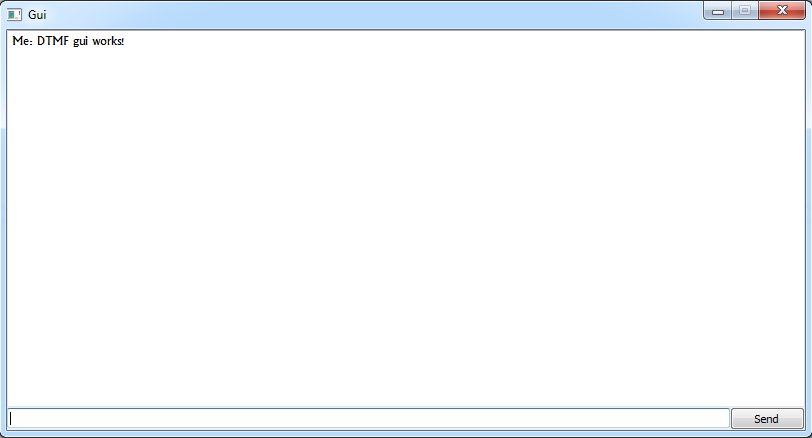
\includegraphics[scale=0.5]{Billeder/GUI.PNG}
	\caption{Den Grafiske Brugerflade}
	\label{fig:tidsplan}
\end{figure}